%%This is a very basic article template.
%%There is just one section and two subsections.
\documentclass{article}
\usepackage[utf8]{inputenc}
\usepackage{a4wide}
\usepackage{german, amsfonts, amssymb, amsmath, ulem, amsthm, amstext}
\usepackage{enumerate}
%\usepackage[latin1]{inputenc}
\usepackage{caption,graphicx,wrapfig}
\usepackage{gauss}
\setcounter{tocdepth}{4}   %= Aufnahme in das Inhaltsverzeichnis *
\setcounter{secnumdepth}{4}  % = Nummerierung vertiefen *
\usepackage{graphicx}

\newcommand{\dpP}{\partial \Phi}
\newcommand{\dpXi}{\partial \xi}
\newcommand{\dpEta}{\partial \eta}
\newcommand{\dpX}{\partial x}
\newcommand{\dpY}{\partial y}
% ä ö includen
% TODO am ende \mathbf vor jedes Phi
  
\begin{document}

\title{Pratkikumsbericht zur Vorlesung \\Numerische Strömungssimulation}
\author{Thomas Camminaidy (297538), Peter Collienne (296711)}
\date{\today}
\maketitle \newpage

\tableofcontents \newpage


\section{Einleitung}
Der Vorliegende Bericht fasst die Inhalte des Programmierpraktikums zur Vorlesung Numerische Strömungssimulation 
im Sommersemester 2012 bei Dr.-Ing. Bernd Binninger zusammen. Die
Programmieraufgaben lassen sich in vier Themen unterteilen die in diesem Bericht enthalten sind. Ziel des Praktikums war es einen eigenen Strömungslöser mit Gittergenierirung zu implementieren und anhand verschiedener Testfälle zu validieren.
Zuerst befassten wir uns mit der Potentialströmung und einem passenden Lösungsverfahren. Anschließend fertigten wir einen 
Gittergenerator an, den wir im nächsten Schritt als Grundlage für die Lösung der Konvektions-Diffusions-Gleichung 
und anschließend der Impulsgleichung verwendet haben.


\section{Potentialströmung}
Potentialströmungen beschreiben das Strömungsfeld unter der Annahme einer inkompressiblen, reibungsfreien, wirbelfreien, zweidimensionalen
Strömung. Die Geschwindigkeiten des Fluids ergeben sich dann als Ableitung der Potential- bzw. Stromfunktion.
\begin{align} u =\frac{ \partial \Phi} {\partial x} \text{ und } v =\frac{ \partial \Phi} {\partial y}\end{align}
Mit Hilfe dieser Beschreibung der Geschwindigkeiten und unter Anwendung der Kontinuitätsgleichung 
lässt sich dann die 
2D-Laplace Gleichung für die Potentialfunktion $\Phi$ beschreiben.
Ausgangspunkt für die Beschreibung der Strömung ist die Kontinuitätsgleichung, welche unter Berücksichtigung von (1) eine 2D-Laplace Gleichung für die 
Potentialfunktion $\Phi$ darstellt.
\begin{align} &\nabla \cdot \mathbf{v} =0 \\ \Leftrightarrow &\frac{ \partial u} {\partial x}+ \frac{ \partial v} {\partial y}=0
\\ \Leftrightarrow &\Delta \Phi = 0 \end{align}
Neben der Potentialfunktion erfüllt ebenfalls die Stromfunktion $\Psi$ eine Laplacegleichung. Charakteristisch für Potentialströmungen
ist, dass die Isolinien der Potentialfunktion und Stromfunktion Senkrecht aufeinander stehen. Dies wird im folgenden auch als Kriterium für die
Bewertung unserers Programms benutzt. Zusätzlich zu der Laplacegleichung benötigt eine PDE auch noch Randbedingungen die durch die gegebene Geometrie
und z.B. Haftbedingungen vorgegeben sind.


\subsection{Diskretisierung auf einem äquidistanten orthogonalen Gitter}
Um die Laplacegleichung (2) zu lösen müssen die Ableitungen numerisch mittels finite Differenzen Approximiert werden.
Auf einem äquidistanten lassen sich die Laplacegleichung $\Delta \Phi = 0$ schreiben als
\begin{align}
\frac{\Phi_{i+1,j}-2\Phi_{i,j}+\Phi_{i-1,j}}{\Delta x^2}+\frac{\Phi_{i,j+1}-2\Phi_{i,j}+\Phi_{i,j-1}}{\Delta y^2}=0
\end{align}
Dabei bezeichnet $i$ den Laufindex in x-Richtung, also $x_i = \Delta x \cdot i$ und $j$ analog den Laufindex in y-Richtung.
Um eine Iterationsvorschrift für $\Phi_{i,j}$ zu erhalten, wird Gleichung (5) umgeformt.
\begin{align}
\Phi_{i,j} =\frac{\Delta x^2(\Phi_{i,j+1}+\Phi_{i,j-1})+\Delta y ^2(\Phi_{i+1,j}+\Phi_{i-1,j}) }{2(\Delta x^2 + \Delta y^2)}
\end{align}
Um für die Potentialfunktion zu lösen, iterieren wir mit Vorschrift (6) solange über unser Rechengebiet, bis $\Phi$ auskonvergiert ist.
Das Jacobi- und das Gauß-Seidel-Verfahren sind zwei mögliche Implementierungen. Der Unterschied zwischen den beiden Methoden liegt 
in der Verwendung der benachbarten Gitterpunkte $\Phi_{i\pm1, j\pm1}$. Das Jacobi-Verfahren verwendet dabei die Punkte aus dem Letzten Iterationsschritt,
während das Gauß-Seidel-Verfahren schon im momentanen Zeitschritt aktualisierte Punkte berücksichtigt. Das Gauß-Seidel-Verfahren konvergiert dabei in 
unseren Testfällen deutlich schneller als das Jacobi-Verfahren. Als weitere Option der Konvergenzbeschleunigung lässt sich das Gauß-Seidel-Verfahren 
noch mit einem Relaxationsfaktor versehen, bei dem entweder eine Über- oder eine Unterrelaxation verwendet werden kann.

\subsubsection{Testfall Parallelströmung} 
Zu Beginn wählen wir uns einen möglichst einfachen Testfall. Dazu setzen wir $\Omega =[0,1]^2$ als Einheitsquadrat welches 
wir in 20 Punkte in X-Richtung und 20 Punkte in Y-Richtung aufteilen. Als Fehlertoleranz setzen wir $\epsilon= 1e-6$.
und setzen das Potential am linken Rand fest auf $\Phi = 2$ und für den rechten Rand $\Phi = 0$.
Die beiden Grafiken Zeigen die Isolinien der Potential- und Stromfunktion.\\
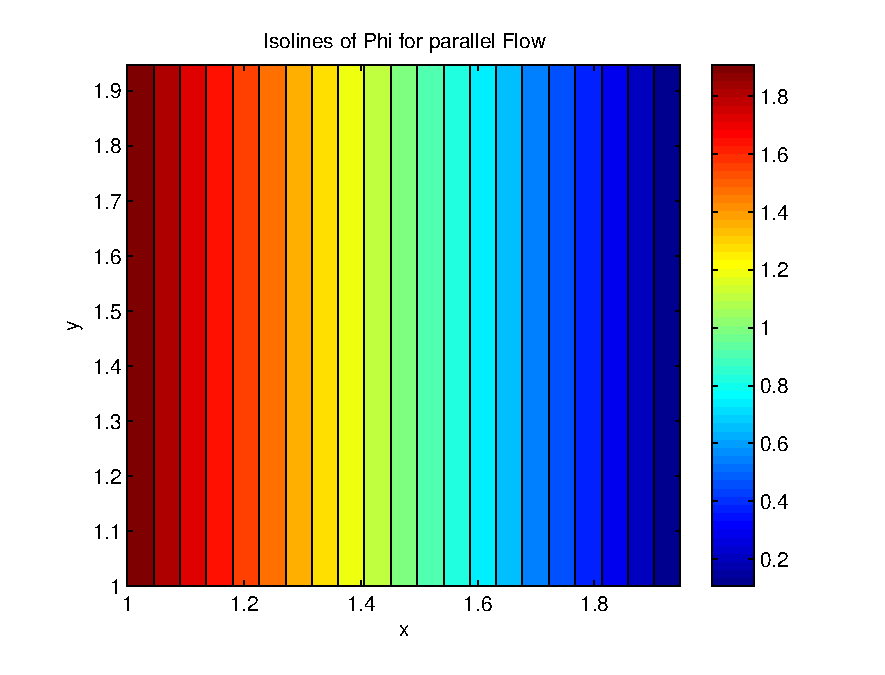
\includegraphics[scale=0.5]{test/1parallel/phi.eps} 
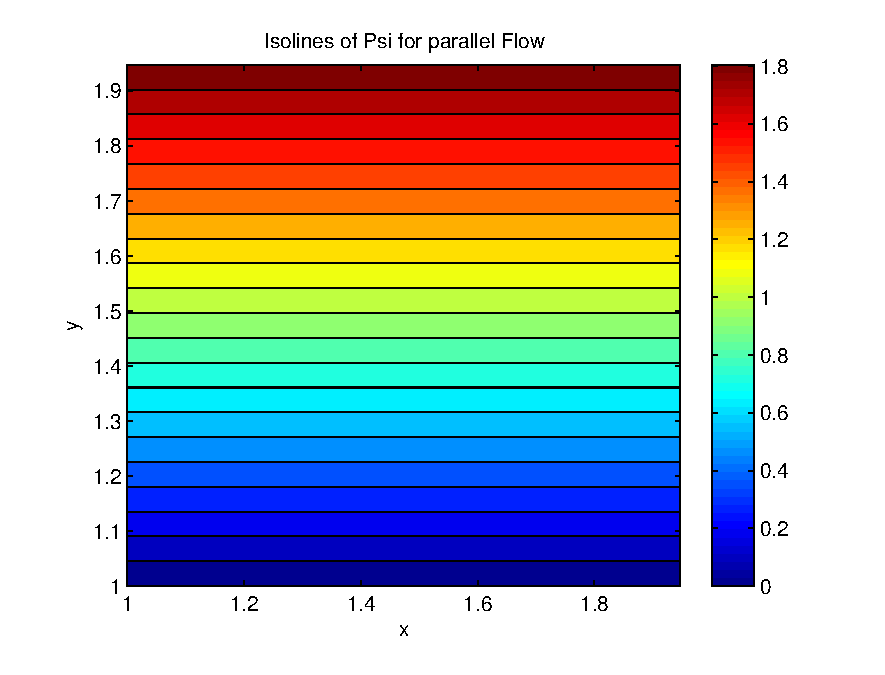
\includegraphics[scale=0.5]{test/1parallel/psi.eps}  \\
Die folgende Grafik legt die Isolinien von Psi und Phi übereinander. Es zeigt sich, dass diese wie
gefordert senkrecht aufeinander stehen.\\ 
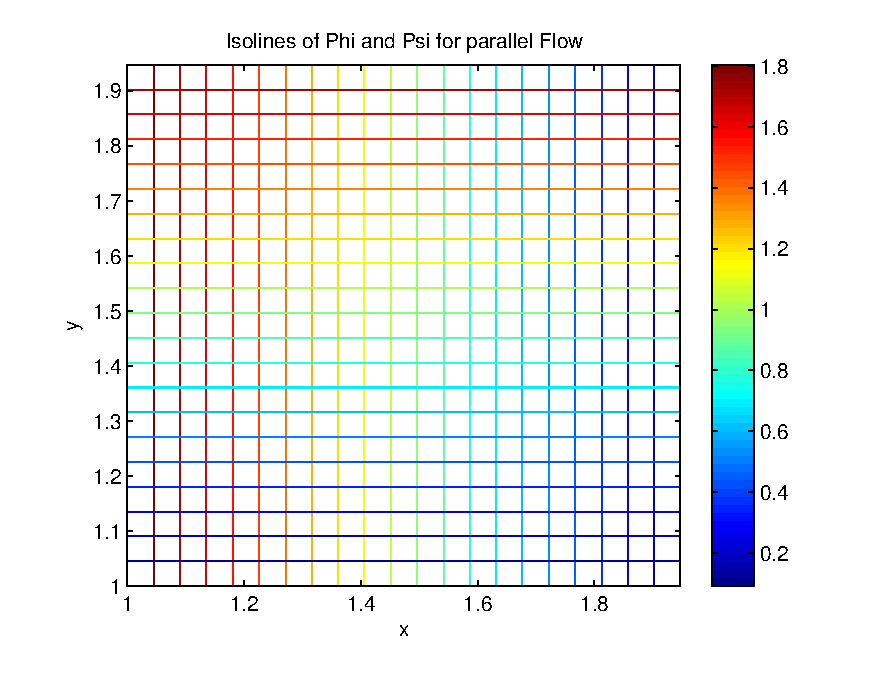
\includegraphics[scale=0.6]{test/1parallel/both.eps}\\
Das Gauß-Seidel-Verfahren konvergiert nach 1079 Schritten. Im nachstehenden Plot ist zu sehen, dass die Konvergenzgeschwindigkeit
mit zunehmender Iterationsanzahl zunimmt. Dieses Phänomen lässt sich an mehreren Testefällen vorfinden.\\
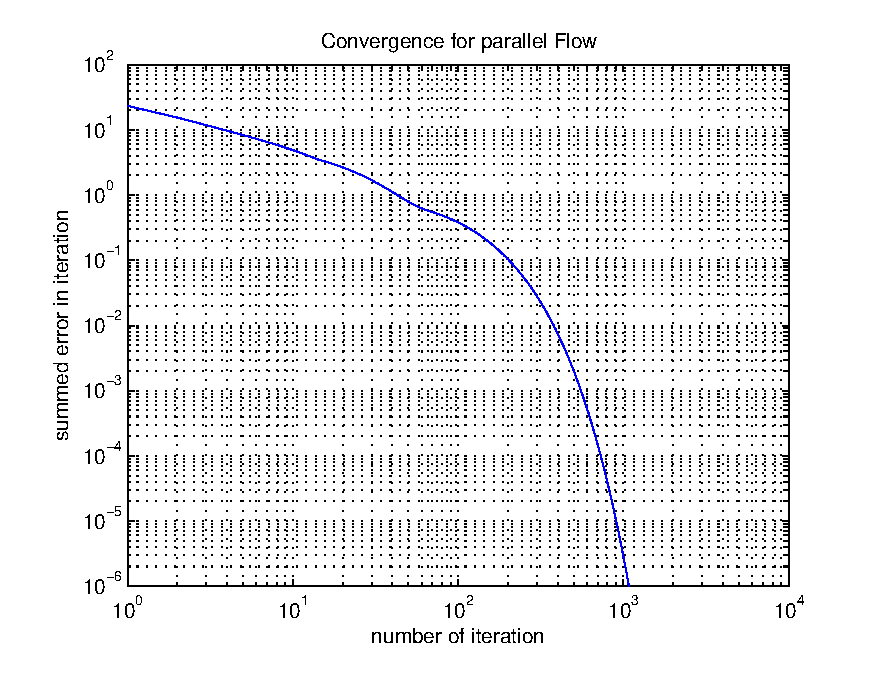
\includegraphics[scale=0.7]{test/1parallel/error.eps}

\subsubsection{Testfall Wirbel}
Als zweiten Testfall haben wir die Potentialfunktion für einen Wirbel gewählt.
Das Gebiet für diesen Fall ist $\Omega =[1,2]^2$ mit erneut 20 Punkten pro Dimension. 
Der Wirbelmittelpunkt befindet sich im Punkt
$(0,0)$. Das Potential für einen Wirbel ergibt sich zu
\begin{align}
\Phi = \frac{E}{2\pi}\arctan\Bigl(\frac{y}{x}\Bigr)
\end{align}
Analog ergibt sich die Stromfunktion zu
\begin{align}
\Psi = -\frac{E}{2\pi}\sqrt{{y}^2+{x}^2}
\end{align}
Der Wirbelmittelpunkt wurde bewusst außerhalb des Gebietes gewählt, da 
mit der obigen Iterationsorschrift für $\Phi$ nur endliche Werte erzeugt werden;
im Wirbelmittelpunkt hat das Potential allerdings eine Singularität. In unserem Fall
haben wir $\frac{E}{2\pi}=1$ gewählt.
Zu sehen sind erneut die Isolinien der Potential- und Stromfunktion.\newpage
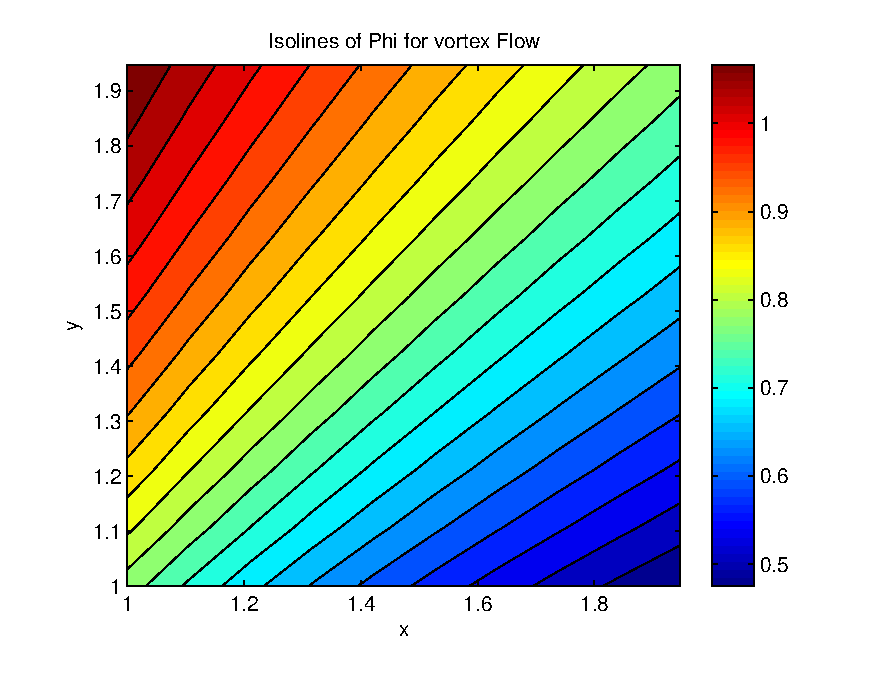
\includegraphics[scale=0.4]{test/2vortex/phi.eps}
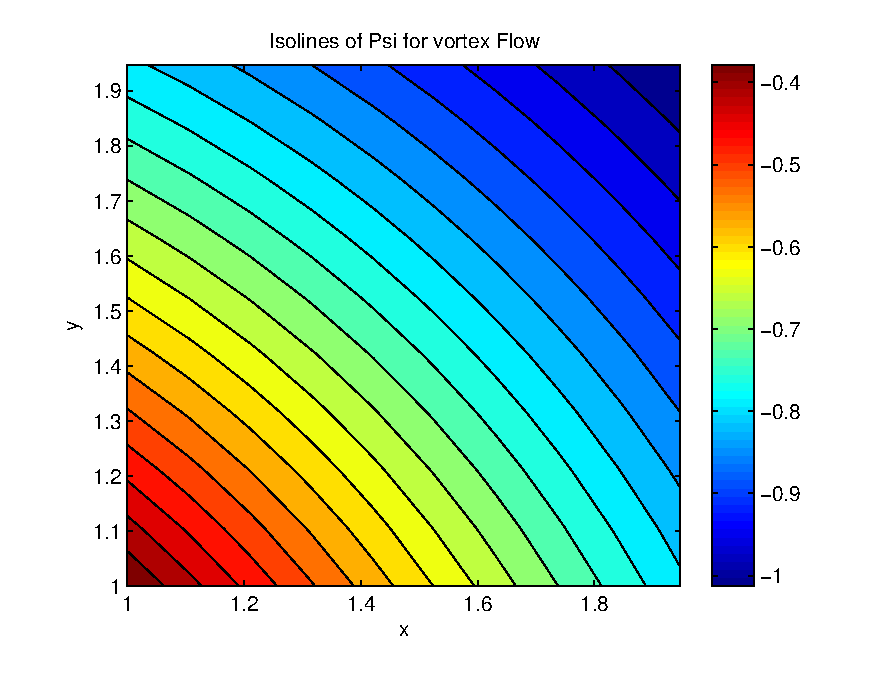
\includegraphics[scale=0.4]{test/2vortex/psi.eps}\\
Im folgenden sind die Isolinien überlagert. Es wird auch hier deutlich,
dass diese senkrecht aufeinander stehen.\\
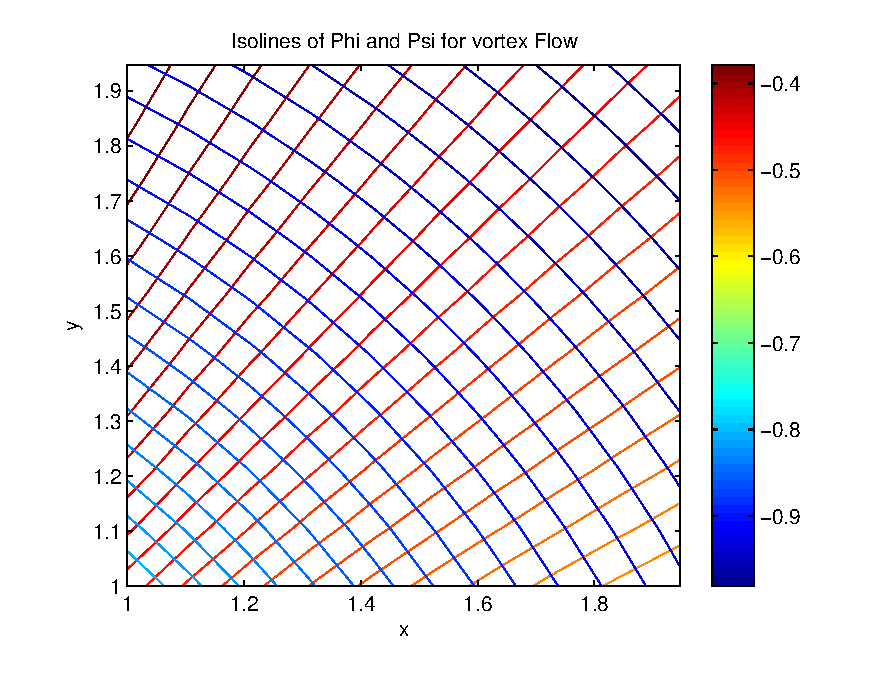
\includegraphics[scale=0.6]{test/2vortex/both.eps}\\
Die Relaxation erstellt in jedem Iterationsschritte die Lösung im Folgeschritt als Linearkombination aus der Lösung im letzten Schritt
und dem aktuellen Schritt.
\begin{align}
\Phi^{k} = \Phi^{k-1} + \beta (\Phi^{\tilde{k}}-\Phi^{k-1})
\end{align}
Für Die Iteration wurden unterschiedliche Werte für den Relaxationsfaktor gewählt. Dabei sieht man signifikante
Unterschiede in der Anzahl der benötigten Iterationsschritte.
So benötigt das Gauß-Seidel-Verfahren ohne Relaxation 601 Iterationsschritte um die Toleranz von $\epsilon 1e-6$ 
zu erreichen. Wesentlich schneller konvergiert das Verfahren für $\beta = 1.8$. Zusätzlich sind noch die Fehlerplots
für $\beta = 0.9$, $\beta = 1.3$, $\beta = 1.9$ beigefügt.

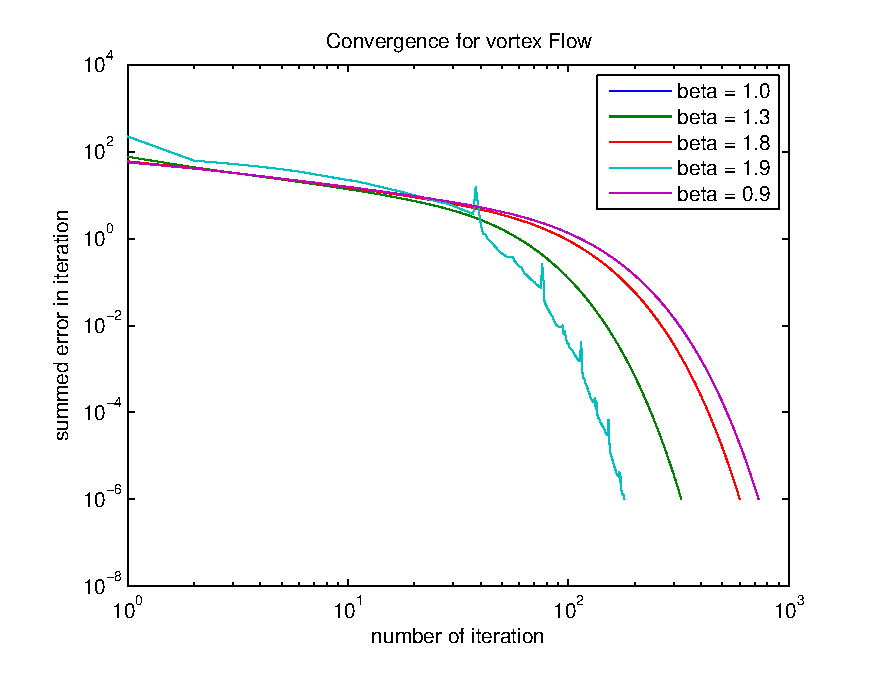
\includegraphics[scale=0.5]{test/2vortex/allerror.eps}


\subsection{Diskretisierung auf einem äquidistanten krummlinigen Gitter}
Da in der Realität die Geometrie der Objekte wesentlich komplexer ist, kommt es fast immer zu krummlinigen Integrationsgebieten.
Um die Laplacegleichung aber weiter wie gewohnt lösen zu können, versucht man, die physikalische Ebene auf ein rechteckiges Rechengebiet
zu transformieren. Dabei transformieren wir die Koordinaten von der $x-y-$Ebene in die $\xi-\eta-$Ebene des Rechengebietes. Wodurch sich folgende
Beziehungen ergeben
\begin{align}
&x = x(\xi,\eta) \ &y = y(\xi,\eta)\\
&\xi=\xi(x,y) \  &\eta=\eta(x,y)  
\end{align}
Durch diese Abhängigkeiten, ergeben sich beim Berechnen der 2. Ableitungen für die Laplacegleichung zusätzliche Terme,
resultierend aus der Kettenregel.
Somit transformiert man die Laplacegleichung zu
\begin{align}
\Bigl( \alpha_1 \frac{\partial^2}{\partial \xi^2} 
+\alpha_2 \frac{\partial^2}{\partial \eta^2} 
+\alpha_3\frac{\partial^2}{\partial \xi \partial \eta}
+\alpha_4 \frac{\partial}{\partial \xi} 
+\alpha_5 \frac{\partial}{\partial \eta} +\alpha_6 \Bigr ) \Phi=0
\end{align}
wobei $\alpha_{1},\ldots,\alpha_{6}$ aus den Ableitungen der Beziehungen in (7) und (8) und der gegebenen Geometrie
resultieren.
Dabei wird einfacheitshalber auf ein Rechengebiet transformiert für das $\Delta \xi=\Delta \eta=1$ gilt.
Somit ergibt sich analog zu (6) die Iterationsvorschrift für $\Phi_{i,j}$ auf einem krummlinigen Gitter zu
\begin{align}
8(\alpha_1+\alpha_2)\Phi_{i,j}  
&= \Phi_{i-1,j-1} \alpha_3 \\
&+\Phi_{i,j-1}(4\alpha_2-2\alpha_5) \notag \\
&-\Phi_{i+1,j-1} \alpha_3 \notag \\
&+\Phi_{i-1,j} (4\alpha_1-2\alpha_4)\notag  \\
&+\Phi_{i+1,j} (4\alpha_1+2\alpha_4)\notag  \\
&-\Phi_{i-1,j+1} \alpha_3\notag  \\
&+\Phi_{i,j+1} (4\alpha_2+2\alpha_5)\notag \\
&+\Phi_{i+1,j+1}\alpha_3 \notag 
\end{align}
\subsubsection{Randbedingungen}
\paragraph{Einström- und Ausströmränder}
$~~$\\
Als Randbedingungen für Ein- und Austrittsrand genügt ein einfaches Geschwindigkeitsprofil, dass durch Integration
in eine passende Randbedingung für die Potentialgleichung überführt werden kann.
In unseren Testfällen beschreiben wir das parallele Einströmen des Fluids in unsere Geometrie,
weshalb das Potential an Ein- und Austrittsrand jeweils konstant gesetzt wird.
\paragraph{Undurchlässige Wände}
$~~$\\
Auf dem Rand folgt die Strömung der Kontur, da die Potentialströmung eine reibungsfreie Strömung beschreibt.
Deshalb gilt auf dem Rand 
\begin{align}
\frac{dh}{dx} = \frac{v}{u} = \frac{\partial \Phi}{\partial y}\Bigl(\frac{\partial \Phi}{\partial x}\Bigr)^{-1}
\end{align}
Somit folgt für den transformierten Raum
\begin{align}
\frac{dh}{dx} = \Bigl(\frac{\dpP}{\dpEta}\frac{\dpEta}{\dpY}+ \frac{\dpP}{\dpEta}\frac{\dpEta}{\dpY}\Bigr)
\Bigl(\frac{\dpP}{\dpEta}\frac{\dpEta}{\dpX}+ \frac{\dpP}{\dpEta}\frac{\dpEta}{\dpX}\Bigr)^{-1}
\end{align}
Statt der Anwendung von zentralen finiten Differenzen muss am $\eta-$Rand auf die Formulierung mittels einseitiger finiter Differenzen
zurückgegriffen werden. Einsetzen der einseitigen Differenzen in $\eta-$Richtung in Gleichung (12) liefert eine Vorschrift zur Berechnung von
$\Phi_{0,j}$ bzw $\Phi_{N,j}$.
Die notwendige Ableitung $\frac{dh}{dx}$ wird auch mittels finiter Differenzen aus der vorgegebenen Kontur berechnet.
In der Implementierung wird dann in jedem Iterationsschritt zuerst $\Phi_{0,j}$ und $\Phi_{N,j}$ bestimmt und im Folgenden
die Potentialgleichung für das innere des Gebietes berechnet. 
\subsubsection{Testfall Diffusor}
sage wie man an die alphas kommt
plot
schön bunt
error
\subsubsection{Testfall 2}
\end{document}